\documentclass[11pt,a4paper]{article}

\usepackage[utf8]{inputenc}
\usepackage[T1]{fontenc}
\usepackage[brazil]{babel}
\usepackage{lmodern}
\usepackage{microtype}
\usepackage[margin=2.5cm]{geometry}
\usepackage{amsmath,amssymb,amsthm,bm}
\usepackage{graphicx}
\usepackage{booktabs}
\usepackage{array}
\usepackage{xcolor}
\usepackage{listings}
\usepackage{float}
\usepackage{caption}
\usepackage[shortlabels]{enumitem}
\usepackage{tikz}
\usetikzlibrary{arrows.meta,positioning,fit,calc,matrix,backgrounds}
\usepackage[most]{tcolorbox}
\usepackage[hidelinks]{hyperref}

% Homóglifos citados no texto: o pdflatex não tem fontes cirílicas/gregas carregadas.
% Como são visualmente idênticos às letras latinas, são impressos com elas; o código
% Unicode aparece ao lado no texto.
\DeclareUnicodeCharacter{0430}{a}
\DeclareUnicodeCharacter{043E}{o}
\DeclareUnicodeCharacter{0440}{p}
\DeclareUnicodeCharacter{0395}{E}
\DeclareUnicodeCharacter{03B2}{\ensuremath{\beta}}
\DeclareUnicodeCharacter{03BC}{\ensuremath{\mu}}
\DeclareUnicodeCharacter{2192}{\ensuremath{\to}}
\DeclareUnicodeCharacter{2264}{\ensuremath{\le}}
\DeclareUnicodeCharacter{2265}{\ensuremath{\ge}}

\graphicspath{{../results/}}

% ---------------------------------------------------------------- cores e caixas
\definecolor{azul}{HTML}{1F4E79}
\definecolor{azulclaro}{HTML}{DCE8F5}
\definecolor{verde}{HTML}{2E7D32}
\definecolor{verdeclaro}{HTML}{E3F1E4}
\definecolor{laranja}{HTML}{B35C00}
\definecolor{laranjaclaro}{HTML}{FCEBD7}
\definecolor{cinza}{HTML}{F4F4F4}

\newtcolorbox{teoria}[1][]{colback=azulclaro,colframe=azul,fonttitle=\bfseries,
  title={Teoria. #1},breakable,sharp corners=south}
\newtcolorbox{nocodigo}[1][]{colback=verdeclaro,colframe=verde,fonttitle=\bfseries,
  title={No código. #1},breakable,sharp corners=south}
\newtcolorbox{atencao}[1][]{colback=laranjaclaro,colframe=laranja,fonttitle=\bfseries,
  title={Atenção. #1},breakable,sharp corners=south}
\newtcolorbox{exercicios}{colback=cinza,colframe=black!50,fonttitle=\bfseries,
  title={Para verificar o entendimento},breakable}

% ---------------------------------------------------------------- código
\lstset{
  basicstyle=\ttfamily\small,
  keywordstyle=\color{azul}\bfseries,
  commentstyle=\color{verde}\itshape,
  stringstyle=\color{laranja},
  backgroundcolor=\color{cinza},
  frame=single, rulecolor=\color{black!20},
  breaklines=true, columns=fullflexible, keepspaces=true,
  showstringspaces=false, language=Python,
  literate={á}{{\'a}}1 {à}{{\`a}}1 {â}{{\^a}}1 {ã}{{\~a}}1 {é}{{\'e}}1 {ê}{{\^e}}1
           {í}{{\'i}}1 {ó}{{\'o}}1 {ô}{{\^o}}1 {õ}{{\~o}}1 {ú}{{\'u}}1 {ç}{{\c c}}1
           {Á}{{\'A}}1 {É}{{\'E}}1 {Ç}{{\c C}}1 {—}{{---}}1 {→}{{$\to$}}1
}

% ---------------------------------------------------------------- matemática
\newcommand{\R}{\mathbb{R}}
\newcommand{\softmax}{\operatorname{softmax}}
\newcommand{\LN}{\operatorname{LN}}
\newcommand{\E}{\mathbb{E}}
\DeclareMathOperator*{\argmax}{arg\,max}
\newtheorem{definicao}{Definição}

\title{\textbf{Mini-GPT Médico}\\[4pt]
\large Relatório de estudo: da tokenização ao treino de um Transformer\\
com questões do Revalida e do Enare}
\author{Projeto em grupo, baseado no nanoGPT de Andrej Karpathy}
\date{Setembro de 2026}

\begin{document}
\maketitle

\begin{abstract}
\noindent Este relatório descreve, passo a passo, a construção de um modelo de linguagem do tipo GPT, escrito do zero em PyTorch e treinado com 5.632 questões de provas médicas brasileiras. O modelo prevê o próximo \emph{caractere} de um texto. Cada etapa do projeto (dados e tokenização, arquitetura, treino, geração e experimentos) é apresentada em três camadas: a \textbf{teoria} que a justifica, com referência aos livros-texto; o \textbf{código} que a implementa; e os \textbf{números} obtidos. O modelo base, com 833.661 parâmetros, reduz a perda de validação de 4,90 para 1,25 nats por caractere em 13 minutos de CPU e aprende o formato das questões, mas não o conteúdo médico. Uma comparação honesta com modelos de $n$-gramas mostra que, com esse orçamento de treino, um modelo de 6-gramas (1,14) ainda o supera. Na Seção~\ref{sec:experimentos}, um modelo 5,8 vezes maior, treinado pelo mesmo número de passos, chega a 1,12 e passa o 6-grama por pouco.
\end{abstract}

\tableofcontents
\newpage

% =====================================================================
\section{Como ler este relatório}
% =====================================================================

O projeto tem cinco etapas, e cada uma virou um arquivo do repositório:

\begin{center}
\begin{tabular}{@{}llll@{}}
\toprule
Etapa & O que faz & Arquivo & Seção \\
\midrule
1. Dados e tokenização & texto $\to$ números & \texttt{data/prepare.py} & \ref{sec:dados} \\
 & & \texttt{char\_tokenizer.py} & \\\
2. Arquitetura & números $\to$ probabilidades & \texttt{model.py} & \ref{sec:arquitetura} \\
3. Treino & ajusta os pesos & \texttt{train.py} & \ref{sec:treino} \\
4. Geração e avaliação & probabilidades $\to$ texto & \texttt{generate.py} & \ref{sec:geracao} \\
5. Experimentos & compara configurações & \texttt{configs/}, \texttt{compare.py} & \ref{sec:experimentos} \\
\bottomrule
\end{tabular}
\end{center}

A Figura~\ref{fig:pipeline} mostra o caminho completo. Ao longo do texto aparecem três tipos de caixa: \textcolor{azul}{\textbf{Teoria}} (o que os livros dizem), \textcolor{verde}{\textbf{No código}} (onde a ideia aparece no projeto) e \textcolor{laranja}{\textbf{Atenção}} (armadilhas e erros que de fato aconteceram). Cada seção termina com perguntas para conferir o entendimento.

\begin{figure}[H]
\centering
\begin{tikzpicture}[
  caixa/.style={draw, rounded corners, fill=azulclaro, minimum height=1.1cm, text width=2.2cm, align=center, font=\small},
  seta/.style={-{Stealth[length=2.5mm]}, thick}]
\node[caixa] (a) {HealthQA-BR\\5.632 questões};
\node[caixa, right=0.4cm of a] (b) {Limpeza e\\formatação\\\scriptsize\texttt{prepare.py}};
\node[caixa, right=0.4cm of b] (c) {Tokenização\\125 símbolos\\\tiny\texttt{char\_tokenizer.py}};
\node[caixa, right=0.4cm of c] (d) {Lotes $(x, y)$\\\scriptsize\texttt{loader.py}};
\node[caixa, below=1.2cm of d, fill=verdeclaro] (e) {Transformer\\\scriptsize\texttt{model.py}};
\node[caixa, left=0.4cm of e, fill=verdeclaro] (f) {Perda e\\AdamW\\\scriptsize\texttt{train.py}};
\node[caixa, left=0.4cm of f, fill=laranjaclaro] (g) {Checkpoint\\\scriptsize\texttt{base.pt}};
\node[caixa, left=0.4cm of g, fill=laranjaclaro] (h) {Geração\\\scriptsize\texttt{generate.py}};
\draw[seta] (a) -- (b); \draw[seta] (b) -- (c); \draw[seta] (c) -- (d);
\draw[seta] (d) -- (e); \draw[seta] (e) -- (f); \draw[seta] (f) -- (g); \draw[seta] (g) -- (h);
\draw[seta, dashed] (f.north) to[bend left=35] node[midway, above, font=\scriptsize] {gradientes atualizam os pesos} (e.north west);
\end{tikzpicture}
\caption{O caminho dos dados no projeto. Em azul, a Etapa 1; em verde, as Etapas 2 e 3; em laranja, a Etapa 4.}
\label{fig:pipeline}
\end{figure}

% =====================================================================
\section{Fundamentos: o que é um modelo de linguagem}
\label{sec:fundamentos}
% =====================================================================

\subsection{Texto como sequência e a regra da cadeia}

Um texto é uma sequência de símbolos $x_1, x_2, \dots, x_T$. No nosso caso cada símbolo é um caractere. Um \emph{modelo de linguagem} atribui uma probabilidade a cada sequência. Pela regra da cadeia da probabilidade, que vale para qualquer distribuição,
\begin{equation}
P(x_1, \dots, x_T) = \prod_{t=1}^{T} P(x_t \mid x_1, \dots, x_{t-1}).
\label{eq:cadeia}
\end{equation}
Essa igualdade transforma um problema difícil (dar probabilidade a um texto inteiro) em muitos problemas iguais e mais simples: \textbf{prever o próximo símbolo, dado o que veio antes}. Um modelo que faz isso é chamado de \emph{auto-regressivo}. O GPT é exatamente isso: uma função que recebe um contexto e devolve uma distribuição de probabilidade sobre o próximo caractere.

\begin{teoria}[Regra da cadeia e modelos auto-regressivos]
A regra da cadeia está em \cite[cap.~3]{goodfellow}. Jurafsky e Martin \cite[cap.~3]{jurafsky} usam a Equação~\eqref{eq:cadeia} como ponto de partida para os modelos de $n$-gramas. O que muda entre um modelo de $n$-gramas e um Transformer é \emph{como} se estima $P(x_t \mid x_{<t})$. O $n$-grama conta ocorrências e só olha os $n-1$ símbolos anteriores. O Transformer usa uma rede neural e olha até \texttt{block\_size} símbolos para trás (64, no nosso caso).
\end{teoria}

\subsection{Entropia cruzada: a medida do erro}

Para cada posição $t$, o modelo produz um vetor de probabilidades $\hat{\bm p}_t \in \R^{V}$ sobre os $V = 125$ caracteres. O caractere correto é $y_t$. A perda usada no treino é a \textbf{entropia cruzada}:
\begin{equation}
\mathcal{L} = -\frac{1}{N}\sum_{t=1}^{N} \ln \hat p_t(y_t).
\label{eq:ce}
\end{equation}
Em palavras: a média, sobre todas as posições, de menos o logaritmo da probabilidade que o modelo deu ao caractere certo. Se o modelo dá probabilidade 1 ao certo, a parcela é $-\ln 1 = 0$; se dá probabilidade quase zero, a parcela explode.

\begin{teoria}[Máxima verossimilhança e entropia cruzada]
Minimizar~\eqref{eq:ce} é o mesmo que \textbf{maximizar a verossimilhança} dos dados de treino: o produto~\eqref{eq:cadeia} das probabilidades que o modelo dá ao texto real. Tomar o logaritmo transforma o produto em soma, e o sinal de menos transforma máximo em mínimo. Goodfellow et al. \cite[seção~5.5]{goodfellow} mostram que isso equivale a minimizar a divergência de Kullback--Leibler entre a distribuição dos dados e a do modelo. A unidade de~\eqref{eq:ce} é o \emph{nat}, porque usamos $\ln$. Dividindo por $\ln 2$, obtemos \emph{bits por caractere} \cite[cap.~2]{cover}.
\end{teoria}

\paragraph{Duas formas de interpretar um valor de perda.}
\begin{itemize}
\item \textbf{Probabilidade média no caractere certo:} $e^{-\mathcal{L}}$ é a média geométrica das probabilidades $\hat p_t(y_t)$. Com $\mathcal{L}=1{,}25$, isso dá $e^{-1{,}25}\approx 0{,}29$: o modelo põe, em média, 29\% de probabilidade no caractere certo.
\item \textbf{Perplexidade:} $\mathrm{PPL} = e^{\mathcal{L}}$. Com $\mathcal{L}=1{,}25$, $\mathrm{PPL}\approx 3{,}5$: o modelo fica tão incerto quanto alguém escolhendo ao acaso entre 3 ou 4 caracteres igualmente prováveis. Jurafsky e Martin \cite[cap.~3]{jurafsky} usam a perplexidade como principal métrica de modelos de linguagem.
\end{itemize}

\subsection{O ponto de partida: a perda de um modelo que não sabe nada}
\label{sec:lnv}

Um modelo recém-criado, sem informação nenhuma, deveria dar a mesma probabilidade $1/V$ a todos os caracteres. Nesse caso, cada parcela de~\eqref{eq:ce} vale $-\ln(1/V) = \ln V$, e
\[
\mathcal{L}_{\text{inicial}} = \ln V = \ln 125 \approx 4{,}83 \text{ nats}.
\]
Esse número é o nosso \textbf{primeiro teste de sanidade}: se a primeira perda medida for muito diferente de 4,83, há erro na inicialização ou na ligação entre as camadas. Nosso modelo começou em 4,90 (Seção~\ref{sec:init}).

\subsection{Softmax: de notas para probabilidades}

A rede não produz probabilidades diretamente. Ela produz um vetor de \emph{logits} $\bm z \in \R^V$, uma ``nota'' real para cada caractere. A função softmax transforma as notas em probabilidades:
\begin{equation}
\softmax(\bm z)_i = \frac{e^{z_i}}{\sum_{j=1}^{V} e^{z_j}}.
\label{eq:softmax}
\end{equation}
Os valores ficam entre 0 e 1 e somam 1. Somar a mesma constante a todos os logits não muda o resultado. Com softmax e entropia cruzada juntos, o gradiente da perda em relação aos logits tem uma forma muito simples \cite[seção~6.2.2.3]{goodfellow}:
\begin{equation}
\frac{\partial \mathcal{L}_t}{\partial \bm z} = \hat{\bm p} - \bm e_{y},
\label{eq:gradsoftmax}
\end{equation}
em que $\bm e_y$ é o vetor com 1 na posição do caractere certo e 0 nas demais. O treino ``empurra para cima'' a nota do caractere certo e ``empurra para baixo'' as outras, em proporção à probabilidade que cada uma recebeu.

\begin{exercicios}
\begin{enumerate}
\item Se o vocabulário tivesse 60 caracteres, qual seria a perda inicial esperada?
\item Um modelo tem perda de validação 1,81 bits por caractere. Quanto é isso em nats? E a perplexidade?
\item Derive~\eqref{eq:gradsoftmax} a partir de~\eqref{eq:ce} e~\eqref{eq:softmax}. Dica: derive $\ln\softmax(\bm z)_y$ em relação a $z_i$, separando os casos $i=y$ e $i\neq y$.
\end{enumerate}
\end{exercicios}

% =====================================================================
\section{Etapa 1: dados e tokenização}
\label{sec:dados}
% =====================================================================

\subsection{O conjunto de dados}

Usamos o HealthQA-BR \cite{healthqa}: 5.632 questões de múltipla escolha do Revalida, do Enare Residência Médica e do Enare Multiprofissional, em português, com licença CC-BY 4.0. O \texttt{prepare.py} transforma cada questão num bloco de texto com um cabeçalho:

\begin{lstlisting}[language={},basicstyle=\ttfamily\footnotesize]
### Enare Residência Médica 2024 | Neurocirurgia
Existem vários tipos de osteotomia para o manejo do desequilíbrio sagital e
coronal da coluna vertebral. [...]
(A) 4-8 graus;
(B) 15-20 graus;
[...]
Gabarito: A
\end{lstlisting}

O cabeçalho \texttt{\#\#\# Prova Ano | Área} dá estrutura ao corpus. Como todo bloco começa assim, o modelo aprende que depois de \texttt{\#\#\# Revalida} vem um ano, depois uma área, depois um enunciado. Na geração, basta dar esse começo para o modelo escrever uma questão.

\subsection{Limpeza: por que cada caractere importa}

Com tokenização por caractere, cada símbolo distinto vira uma classe que o modelo precisa aprender a prever. Símbolos inúteis ou duplicados desperdiçam capacidade do modelo e dados de treino. A função \texttt{limpar} aplica, nesta ordem:

\begin{enumerate}
\item \textbf{Normalização Unicode NFC.} Em Unicode, ``é'' pode ser escrito como um caractere só (U+00E9) ou como ``e'' seguido de um acento combinante (U+0065 U+0301). Visualmente são iguais, mas para o tokenizador seriam sequências diferentes. A forma NFC junta tudo na versão de um caractere.
\item \textbf{Substituições de símbolos equivalentes.} Aspas curvas viram retas, travessões viram hífen, espaços especiais viram espaço comum, subscritos viram dígitos (O$_2$ $\to$ O2, como no resto do corpus).
\item \textbf{Homóglifos.} O texto original foi copiado de PDFs e contém letras gregas e cirílicas \emph{visualmente idênticas} às latinas: ``Allium ceра'' com ``р'' cirílico (U+0440), alternativa ``Ε'' escrita com épsilon grego (U+0395). Sem tratamento, ``o'' latino (U+006F) e ``о'' cirílico (U+043E) seriam dois tokens diferentes, e o modelo teria que aprender duas vezes a mesma letra. O mapeamento \texttt{HOMOGLIFOS} troca 27 desses caracteres pelos latinos.
\item \textbf{Espaços e quebras de linha repetidos} são reduzidos.
\item \textbf{Formato das alternativas.} No dataset, as alternativas vinham como dicionário Python (\texttt{'A': 'texto'}), às vezes quebradas em várias linhas. Uma expressão regular as converte em \texttt{(A) texto}, numa linha só.
\item \textbf{Caracteres raros} (menos de 3 ocorrências no corpus inteiro) são removidos. Foram 17, como \texttt{\$}, \texttt{\textasciicircum}, \texttt{®}, \texttt{½} e \texttt{ñ}. Um símbolo que aparece 1 ou 2 vezes não pode ser aprendido e só aumenta o vocabulário.
\end{enumerate}

Resultado: o vocabulário caiu de 144 para \textbf{125 caracteres}. São 80 letras (maiúsculas, minúsculas e acentuadas), dígitos, pontuação e alguns símbolos médicos (\texttt{°}, \texttt{±}, \texttt{≤}, \texttt{≥}, \texttt{β}, \texttt{μ}, \texttt{→}).

\begin{atencao}[Um erro real que a limpeza revelou]
O código da Etapa 1 foi escrito antes de ser rodado com o dataset verdadeiro. Ao rodar, apareceram os homóglifos e o formato de dicionário das alternativas, que ninguém tinha previsto. A lição: \textbf{sempre olhe os dados reais}, por exemplo imprimindo o vocabulário e procurando caracteres estranhos. Ver os 144 caracteres impressos foi o que mostrou letras gregas no meio de palavras em português.
\end{atencao}

\subsection{Separação em treino e validação}

Separamos 90\% das questões para treino e 10\% para validação. Dois cuidados:

\begin{itemize}
\item \textbf{Separação por questão, não por caractere.} Se cortássemos o texto contínuo num ponto qualquer, uma questão poderia ficar metade em cada lado, e parte da validação teria sido ``vista'' no treino. Isso é \emph{vazamento de dados}, e faria a perda de validação parecer melhor do que é.
\item \textbf{Embaralhar antes de separar.} As questões vêm ordenadas por prova e ano. Sem embaralhar, a validação teria só as provas mais recentes, e mediríamos a capacidade de generalizar para outro ano, não para questões novas do mesmo tipo.
\end{itemize}

\begin{teoria}[Por que precisamos de um conjunto de validação]
O objetivo não é ir bem no treino: é ir bem em dados \emph{não vistos}. Goodfellow et al. \cite[seção~5.2]{goodfellow} chamam isso de \emph{erro de generalização}. A perda de treino mede o quanto o modelo se ajusta aos dados que viu. A perda de validação estima o erro em dados novos. Quando a de treino continua caindo e a de validação para de cair ou sobe, o modelo começou a \emph{decorar} (overfitting).
\end{teoria}

\begin{table}[H]
\centering
\begin{tabular}{@{}lr@{}}
\toprule
Medida & Valor \\
\midrule
Questões (treino / validação) & 5.069 / 563 \\
Caracteres de treino / validação & 4.574.978 / 508.218 \\
Tamanho do corpus & 5,25 MB \\
Vocabulário & 125 caracteres \\
Perda inicial esperada, $\ln 125$ & 4,83 nats \\
Caracteres mais frequentes & espaço (14,2\%), a (9,9\%), e (8,8\%), o (7,3\%) \\
\bottomrule
\end{tabular}
\caption{O corpus depois do \texttt{prepare.py}.}
\label{tab:corpus}
\end{table}

\subsection{Tokenização em nível de caractere}

\begin{definicao}
Um \emph{tokenizador} é um par de funções: \texttt{encode}, que leva texto a uma lista de inteiros (tokens), e \texttt{decode}, que faz o caminho inverso, com $\texttt{decode}(\texttt{encode}(s)) = s$.
\end{definicao}

Nosso tokenizador é o mais simples possível. Ele ordena os caracteres distintos do corpus e numera de 0 a 124:

\begin{lstlisting}
class CharTokenizer:
    def __init__(self, chars):
        self.chars = sorted(set(chars))   # ordenar: mesmo corpus, mesmo vocabulário
        self.stoi = {ch: i for i, ch in enumerate(self.chars)}  # caractere -> inteiro
        self.itos = {i: ch for i, ch in enumerate(self.chars)}  # inteiro -> caractere

    def encode(self, text):
        return [self.stoi[ch] for ch in text]

    def decode(self, ids):
        return "".join(self.itos[int(i)] for i in ids)
\end{lstlisting}

\paragraph{Por que caractere, e não palavra ou sub-palavra?} Há um compromisso entre o tamanho do vocabulário e o comprimento das sequências:

\begin{center}
\begin{tabular}{@{}lccc@{}}
\toprule
Nível & Vocabulário & Sequência & Palavras nunca vistas \\
\midrule
Caractere & pequeno (125) & longa & impossíveis: tudo é soletrável \\
Sub-palavra (BPE) & médio (milhares) & média & raras \\
Palavra & enorme (dezenas de milhares) & curta & frequentes \\
\bottomrule
\end{tabular}
\end{center}

O GPT-2 e seus sucessores usam BPE (\emph{byte-pair encoding}) \cite{sennrich}, que junta os pares de símbolos mais frequentes até atingir um vocabulário de dezenas de milhares de tokens. Escolhemos caracteres porque o código fica curto e fácil de explicar, o vocabulário é pequeno (a camada de saída tem só 125 classes) e o modelo nunca encontra uma palavra desconhecida. O custo é que o modelo precisa aprender a \emph{soletrar}, e o contexto de 64 tokens cobre só cerca de 10 palavras.

\begin{atencao}[O conflito de nomes com o pacote \texttt{tokenizer}]
O arquivo se chamava \texttt{tokenizer.py}. Existe um pacote no pip com o mesmo nome (um tokenizador de islandês). Quando ele estava instalado e o código rodava fora da raiz do projeto, como num notebook aberto em \texttt{notebooks/}, o Python importava o pacote do pip no lugar do nosso e dava \texttt{ImportError: cannot import name 'CharTokenizer'}. A solução foi renomear o arquivo para \texttt{char\_tokenizer.py}. Lição: evite nomes de módulo genéricos que podem coincidir com pacotes instalados.
\end{atencao}

\subsection{Armazenamento e formação dos lotes}

Os tokens são gravados em \texttt{train.bin} e \texttt{val.bin} como inteiros sem sinal de 16 bits (\texttt{uint16}, até 65.535, sobra muito para 125 símbolos). No treino, \texttt{np.memmap} lê o arquivo do disco sob demanda, sem carregar tudo na memória.

Um lote é formado sorteando \texttt{batch\_size} posições iniciais e recortando \texttt{block\_size}$+1$ tokens seguidos a partir de cada uma. A entrada $x$ são os primeiros \texttt{block\_size} tokens; o alvo $y$ é o mesmo trecho \textbf{deslocado uma posição}:

\begin{center}
\begin{tikzpicture}[
  cel/.style={draw, minimum width=1cm, minimum height=0.7cm, font=\ttfamily\small},
  rot/.style={font=\small, anchor=east}]
\foreach \c [count=\i] in {F,e,b,r,e} { \node[cel, fill=azulclaro] at (\i*1.05, 0) {\c}; }
\foreach \c [count=\i] in {e,b,r,e,{\textvisiblespace}} { \node[cel, fill=verdeclaro] at (\i*1.05, -1.1) {\c}; }
\node[rot] at (0.4, 0) {$x$ (entrada)};
\node[rot] at (0.4, -1.1) {$y$ (alvo)};
\foreach \i in {1,...,5} { \draw[-{Stealth}, gray] (\i*1.05, -0.37) -- (\i*1.05, -0.73); }
\node[font=\small, text width=6.3cm, anchor=west] at (6.2, -0.55) {Na posição $t$, o modelo vê $x_1,\dots,x_t$ e precisa prever $y_t = x_{t+1}$.};
\end{tikzpicture}
\end{center}

Um bloco de 64 tokens gera \textbf{64 exemplos de treino ao mesmo tempo}: ``depois de F, vem e'', ``depois de Fe, vem b'', ``depois de Feb, vem r'', e assim por diante. Um lote de $32 \times 64$ gera 2.048 exemplos por passo. Isso só é possível porque a máscara causal (Seção~\ref{sec:mascara}) impede cada posição de ver as seguintes.

\begin{exercicios}
\begin{enumerate}
\item Por que a normalização NFC precisa vir \emph{antes} da contagem de caracteres raros?
\item Se não tivéssemos tratado os homóglifos, o que aconteceria com a perda de um modelo que encontra ``о'' cirílico na validação, mas nunca no treino?
\item Quantos exemplos de previsão existem num lote com \texttt{batch\_size}$=16$ e \texttt{block\_size}$=128$?
\end{enumerate}
\end{exercicios}

% =====================================================================
\section{Uma régua de comparação: modelos de $n$-gramas}
\label{sec:ngramas}
% =====================================================================

Antes de avaliar o Transformer, vale saber quanto um modelo \emph{muito} mais simples consegue. O modelo de $n$-gramas, o modelo de linguagem clássico \cite[cap.~3]{jurafsky}, supõe que o próximo caractere depende só dos $n-1$ anteriores (hipótese de Markov) e estima as probabilidades por contagem:
\begin{equation}
P(x_t \mid x_{t-n+1}, \dots, x_{t-1}) \approx \frac{C(x_{t-n+1}\dots x_t) + \alpha}{C(x_{t-n+1}\dots x_{t-1}) + \alpha V},
\end{equation}
em que $C(\cdot)$ conta ocorrências no treino e $\alpha$ é uma suavização aditiva, que evita probabilidade zero para sequências nunca vistas. Contamos no \texttt{train.bin} e medimos a entropia cruzada no \texttt{val.bin}:

\begin{table}[H]
\centering
\begin{tabular}{@{}lccccccc@{}}
\toprule
$n$ & 1 & 2 & 3 & 4 & 5 & 6 & 7 \\
\midrule
Perda de validação (nats), $\alpha = 0{,}01$ & 3,24 & 2,39 & 1,92 & 1,49 & 1,22 & \textbf{1,14} & 1,19 \\
\bottomrule
\end{tabular}
\caption{Modelos de $n$-gramas por contagem. $n=1$ só conhece a frequência de cada caractere; $n=2$ olha o caractere anterior.}
\label{tab:ngramas}
\end{table}

Duas lições que voltam mais adiante:
\begin{itemize}
\item \textbf{Mais contexto ajuda, até certo ponto.} A perda cai de 3,24 ($n=1$) para 1,14 ($n=6$). Com $n=7$ ela volta a subir: a maioria das sequências de 7 caracteres da validação nunca apareceu no treino, e as contagens ficam esparsas demais. Esse é o problema que os modelos neurais resolvem: em vez de decorar sequências exatas, aprendem representações que \emph{generalizam} para sequências parecidas \cite{bengio2003}.
\item \textbf{A régua é exigente.} Um 6-grama bem suavizado chega a 1,14 nats. Um detalhe torna essa régua um pouco otimista: escolhemos $\alpha$ olhando a própria validação. O Transformer da Seção~\ref{sec:treino} precisa ser comparado com esse número.
\end{itemize}

% =====================================================================
\section{Etapa 2: a arquitetura do Transformer}
\label{sec:arquitetura}
% =====================================================================

\subsection{Encoder, decoder e o que é o GPT}

O Transformer original \cite{vaswani} foi criado para tradução e tem duas torres (Figura~\ref{fig:encdec}). O \emph{encoder} lê a frase de entrada (``That is good'') com atenção bidirecional: cada palavra vê todas as outras. O \emph{decoder} escreve a tradução (``Das ist gut'') uma palavra por vez, com atenção mascarada, e consulta o encoder pela \emph{atenção cruzada}.

O GPT \cite{radford2019} não traduz: ele continua um texto. Não há frase de entrada para o encoder ler, então o GPT usa \textbf{só o decoder, sem a atenção cruzada}. Cada bloco tem apenas atenção mascarada e MLP. Nosso modelo é exatamente isso. Bishop e Bishop \cite[cap.~12]{bishop} apresentam as duas variantes com a mesma notação usada aqui.

\begin{figure}[H]
\centering
\begin{tikzpicture}[
  bloco/.style={draw, rounded corners, minimum width=2.6cm, minimum height=0.6cm, font=\small},
  torre/.style={draw, rounded corners, inner sep=6pt},
  seta/.style={-{Stealth}, thick}]
% encoder
\node[bloco, fill=azulclaro] (eatt) at (0,0) {Atenção bidirecional};
\node[bloco, fill=verdeclaro, above=0.25cm of eatt] (emlp) {MLP};
\node[font=\small, below=0.35cm of eatt] (ein) {That is good};
\begin{scope}[on background layer]
\node[torre, fill=black!5, fit=(eatt)(emlp), label=above:{\small Encoder}] (enc) {};
\end{scope}
% decoder original
\node[bloco, fill=azulclaro] (datt) at (4.6,0) {Atenção mascarada};
\node[bloco, fill=red!15, above=0.25cm of datt] (dcross) {Atenção cruzada};
\node[bloco, fill=verdeclaro, above=0.25cm of dcross] (dmlp) {MLP};
\node[font=\small, below=0.35cm of datt] {[BOS] Das ist gut};
\begin{scope}[on background layer]
\node[torre, fill=black!5, fit=(datt)(dcross)(dmlp), label=above:{\small Decoder (tradução)}] (dec) {};
\end{scope}
\draw[seta] (enc.east) -- (dcross.west);
% GPT
\node[bloco, fill=azulclaro] (gatt) at (9.6,0) {Atenção mascarada};
\node[bloco, fill=verdeclaro, above=0.25cm of gatt] (gmlp) {MLP};
\node[font=\small, below=0.35cm of gatt] {\texttt{\#\#\# Revalida}};
\begin{scope}[on background layer]
\node[torre, fill=verdeclaro!40, fit=(gatt)(gmlp), label=above:{\small\textbf{GPT: só decoder}}] (gpt) {};
\end{scope}
\node[font=\scriptsize, text width=3.2cm, align=center] at (9.6,-1.75) {(bloco repetido $n_{\text{layer}}=4$ vezes)};
\end{tikzpicture}
\caption{À esquerda, o Transformer de tradução \cite{vaswani}. À direita, o GPT: sem encoder e, portanto, sem atenção cruzada.}
\label{fig:encdec}
\end{figure}

\subsection{Visão geral e as dimensões}

Usamos a notação $B$ para o tamanho do lote (32), $T$ para o comprimento do contexto (até 64), $C$ para a dimensão dos vetores internos, \texttt{n\_embd} (128), e $V$ para o vocabulário (125). O caminho de um lote pelo modelo é:
\begin{align*}
\text{ids} \in \{0..V-1\}^{B\times T}
&\;\xrightarrow{\text{embeddings}}\; \bm X^{(0)} \in \R^{B\times T\times C}
\;\xrightarrow{\;4\text{ blocos}\;}\; \bm X^{(4)} \in \R^{B\times T\times C} \\
&\;\xrightarrow{\LN,\ \text{linear}}\; \text{logits} \in \R^{B\times T\times V}.
\end{align*}
A dimensão $C$ fica constante do começo ao fim dos blocos. Isso é o que permite somar a entrada de cada bloco com a saída dele (conexões residuais).

\subsection{Embeddings de token e de posição}

A \emph{embedding de token} é uma tabela $\bm W_{\text{tok}} \in \R^{V\times C}$: o caractere de id $i$ é representado pela linha $i$. É equivalente a multiplicar um vetor \emph{one-hot} pela matriz, mas sem fazer a multiplicação. Os valores da tabela são aprendidos, e caracteres que se comportam de forma parecida, como vogais, tendem a ficar com vetores parecidos.

A atenção, sozinha, não sabe a ordem das posições: se embaralharmos as entradas, as saídas se embaralham do mesmo jeito. Por isso somamos uma \emph{embedding de posição} $\bm W_{\text{pos}} \in \R^{T_{\max}\times C}$, também aprendida, como no GPT-2:
\begin{equation}
\bm X^{(0)}_t = \bm W_{\text{tok}}[x_t] + \bm W_{\text{pos}}[t].
\end{equation}
O Transformer original \cite{vaswani} usava senos e cossenos fixos em vez de uma tabela aprendida. As duas opções funcionam.

\subsection{Atenção causal com várias cabeças}

A atenção é a única parte do modelo em que \textbf{as posições trocam informação}. Todo o resto (embeddings, MLP, LayerNorm) age em cada posição separadamente.

\paragraph{Consulta, chave e valor.} A partir de cada vetor $\bm x_t$, três projeções lineares aprendidas geram:
\begin{align*}
\bm q_t &= \bm W_Q \bm x_t \qquad \text{consulta: ``o que procuro''},\\
\bm k_t &= \bm W_K \bm x_t \qquad \text{chave: ``o que ofereço''},\\
\bm v_t &= \bm W_V \bm x_t \qquad \text{valor: ``o que passo adiante''}.
\end{align*}
A posição $t$ compara sua consulta com a chave de cada posição $s$ pelo produto escalar $\bm q_t \cdot \bm k_s$. Quanto maior o produto, mais a posição $s$ interessa a $t$. Os produtos viram pesos pelo softmax, e a saída é a média dos valores ponderada por esses pesos. Em forma matricial, para uma cabeça com dimensão $d$ \cite{vaswani}:
\begin{equation}
\operatorname{Atenção}(\bm Q, \bm K, \bm V) = \softmax\!\left(\frac{\bm Q \bm K^\top}{\sqrt{d}} + \bm M\right) \bm V .
\label{eq:atencao}
\end{equation}

\paragraph{Por que dividir por $\sqrt d$.} Suponha que as componentes de $\bm q$ e $\bm k$ sejam independentes, com média 0 e variância 1. Então $\bm q\cdot\bm k = \sum_{i=1}^{d} q_i k_i$ é uma soma de $d$ termos de variância 1, e tem variância $d$. Com $d=32$, os produtos teriam desvio padrão $\approx 5{,}7$. Com valores tão espalhados, o softmax fica quase ``one-hot'': uma posição recebe quase todo o peso e o gradiente das outras some. Dividir por $\sqrt d$ traz a variância de volta para 1.

\paragraph{A máscara causal.}
\label{sec:mascara}
A matriz $\bm M$ em~\eqref{eq:atencao} tem 0 onde a posição pode olhar ($s \le t$) e $-\infty$ onde não pode ($s > t$). Como $e^{-\infty} = 0$, o softmax dá peso zero ao futuro. Para $T=4$:
\[
\frac{\bm Q\bm K^\top}{\sqrt d} + \bm M =
\begin{pmatrix}
a_{11} & -\infty & -\infty & -\infty\\
a_{21} & a_{22} & -\infty & -\infty\\
a_{31} & a_{32} & a_{33} & -\infty\\
a_{41} & a_{42} & a_{43} & a_{44}
\end{pmatrix}
\;\xrightarrow{\softmax\text{ por linha}}\;
\begin{pmatrix}
1 & 0 & 0 & 0\\
\ast & \ast & 0 & 0\\
\ast & \ast & \ast & 0\\
\ast & \ast & \ast & \ast
\end{pmatrix}.
\]
Cada linha soma 1. A primeira posição só pode olhar para si mesma. Sem a máscara, a posição $t$ poderia ler $x_{t+1}$, que é exatamente o alvo $y_t$: prever seria copiar, a perda de treino iria a zero e o modelo não aprenderia nada útil para gerar texto.

\paragraph{Várias cabeças.} Em vez de uma atenção com $d = C = 128$, usamos $h=4$ cabeças com $d = C/h = 32$ cada, em paralelo, com projeções independentes. Cada cabeça pode se especializar: uma olha a letra anterior, outra o início da palavra, outra a abertura de um parêntese. As saídas das cabeças são concatenadas e passam por mais uma projeção linear $\bm W_O$. O custo é o mesmo de uma cabeça grande.

\begin{nocodigo}[\texttt{CausalSelfAttention.forward}]
\begin{lstlisting}
q, k, v = self.qkv(x).split(C, dim=2)            # uma camada gera q, k e v
q = q.view(B, T, self.n_head, d).transpose(1, 2)  # (B, n_head, T, d)
# ... o mesmo para k e v
pesos = (q @ k.transpose(-2, -1)) / math.sqrt(d)   # (B, n_head, T, T)
pesos = pesos.masked_fill(self.mascara[:, :, :T, :T] == 0, float("-inf"))
pesos = F.softmax(pesos, dim=-1)                   # futuro recebe peso 0
y = pesos @ v                                       # média ponderada dos valores
y = y.transpose(1, 2).contiguous().view(B, T, C)   # junta as cabeças
return self.resid_dropout(self.proj(y))            # projeção W_O
\end{lstlisting}
A máscara é uma matriz triangular inferior de uns (\texttt{torch.tril}), guardada com \texttt{register\_buffer}: vai junto para a GPU, mas não é um parâmetro treinável. Escrevemos a fórmula à mão, em vez de usar \texttt{F.scaled\_dot\_product\_attention}, para que cada passo de~\eqref{eq:atencao} apareça no código.
\end{nocodigo}

\subsection{MLP, conexões residuais e LayerNorm}

\paragraph{MLP.} Depois de trocar informação pela atenção, cada posição processa sozinha o que recebeu, com uma rede de duas camadas:
\begin{equation}
\operatorname{MLP}(\bm x) = \bm W_2\, \operatorname{GELU}(\bm W_1 \bm x + \bm b_1) + \bm b_2,
\qquad \bm W_1 \in \R^{4C\times C},\ \bm W_2 \in \R^{C\times 4C}.
\end{equation}
A camada interna é 4 vezes mais larga, como em \cite{vaswani}. A ativação GELU \cite{gelu} é $\operatorname{GELU}(x) = x\,\Phi(x)$, em que $\Phi$ é a distribuição acumulada da normal padrão. É uma versão suave da ReLU e é a usada no GPT-2. Sem uma função não linear, as duas camadas lineares equivaleriam a uma só \cite[cap.~6]{goodfellow}. Um bom resumo da divisão de papéis: \textbf{a atenção comunica, o MLP computa}.

\paragraph{Conexões residuais.} Cada subcamada \emph{soma} sua saída à entrada, em vez de substituí-la:
\begin{align}
\bm X' &= \bm X + \operatorname{Atenção}(\LN_1(\bm X)), \label{eq:res1}\\
\bm X'' &= \bm X' + \operatorname{MLP}(\LN_2(\bm X')). \label{eq:res2}
\end{align}
A ideia vem das ResNets \cite{he2016}. Na derivada de~\eqref{eq:res1}, o termo $\bm X$ contribui com a identidade: $\partial \bm X'/\partial \bm X = \bm I + \dots$. Assim o gradiente sempre tem um caminho direto da perda até as primeiras camadas, mesmo que as subcamadas ainda estejam mal ajustadas. Sem isso, redes profundas treinam muito mal.

\paragraph{LayerNorm.} Para cada posição, a LayerNorm \cite{layernorm} padroniza o vetor para média 0 e variância 1 e depois aplica uma escala $\bm\gamma$ e um deslocamento $\bm\beta$ aprendidos:
\begin{equation}
\LN(\bm x) = \bm\gamma \odot \frac{\bm x - \mu}{\sqrt{\sigma^2 + \epsilon}} + \bm\beta,
\qquad \mu = \frac1C\sum_i x_i,\ \ \sigma^2 = \frac1C\sum_i (x_i-\mu)^2.
\end{equation}
Isso mantém os valores numa escala estável, camada após camada. Usamos a LayerNorm \emph{antes} de cada subcamada (``pre-norm'', como no GPT-2 \cite{radford2019}). O artigo original \cite{vaswani} aplicava depois (``post-norm''). O pre-norm deixa o caminho residual limpo e costuma treinar de forma mais estável.

\subsection{A saída do modelo}

Depois dos 4 blocos, uma última LayerNorm e uma camada linear $\bm W_{\text{out}} \in \R^{V\times C}$ produzem os logits de cada posição. A perda compara os logits com os alvos pela entropia cruzada~\eqref{eq:ce}. O PyTorch aplica o softmax dentro de \texttt{F.cross\_entropy}, de forma numericamente estável.

\begin{nocodigo}[\texttt{GPT.forward}]
\begin{lstlisting}
posicoes = torch.arange(T, device=ids.device)
x = self.drop(self.tok_emb(ids) + self.pos_emb(posicoes))  # (B, T, C)
for bloco in self.blocks:
    x = bloco(x)
logits = self.head(self.ln_f(x))                           # (B, T, V)
perda = F.cross_entropy(logits.view(B * T, -1), alvos.view(B * T))
\end{lstlisting}
\end{nocodigo}

\subsection{Contando os parâmetros}

Contar à mão é um ótimo exercício para entender a arquitetura. Uma camada linear de $n$ entradas para $m$ saídas tem $mn$ pesos e $m$ vieses; uma LayerNorm de dimensão $C$ tem $2C$ parâmetros ($\bm\gamma$ e $\bm\beta$). Com $C=128$, $V=125$, $T_{\max}=64$:

\begin{table}[H]
\centering
\begin{tabular}{@{}llr@{}}
\toprule
Parte & Fórmula & Parâmetros \\
\midrule
Embedding de token & $VC$ & 16.000 \\
Embedding de posição & $T_{\max}C$ & 8.192 \\
\midrule
\multicolumn{3}{@{}l}{\emph{Um bloco:}} \\
\quad LayerNorm 1 e 2 & $2\times 2C$ & 512 \\
\quad $\bm W_Q, \bm W_K, \bm W_V$ (juntas) & $C\cdot 3C + 3C$ & 49.536 \\
\quad Projeção $\bm W_O$ & $C^2 + C$ & 16.512 \\
\quad MLP & $(C\cdot 4C + 4C) + (4C\cdot C + C)$ & 131.712 \\
\quad Total do bloco & $12C^2 + 13C$ & 198.272 \\
Quatro blocos & $4\times 198.272$ & 793.088 \\
\midrule
LayerNorm final & $2C$ & 256 \\
Camada de saída & $CV + V$ & 16.125 \\
\midrule
\textbf{Total} & & \textbf{833.661} \\
\bottomrule
\end{tabular}
\caption{Contagem de parâmetros do modelo base. O total bate com \texttt{modelo.num\_parametros()}.}
\label{tab:parametros}
\end{table}

Observe que 95\% dos parâmetros estão nos blocos, e cada bloco tem $\approx 12C^2$. Por isso o número de parâmetros cresce com o \emph{quadrado} de $C$: dobrar \texttt{n\_embd} multiplica o tamanho dos blocos por 4.

\subsection{Inicialização e a perda inicial}
\label{sec:init}

Todos os pesos das camadas lineares e das embeddings começam sorteados de uma normal com média 0 e desvio padrão 0,02, e todos os vieses começam em zero, como no GPT-2. Com pesos pequenos, os logits iniciais ficam perto de zero, o softmax fica quase uniforme e a perda fica perto de $\ln V$.

Ela não fica \emph{exatamente} em $\ln V$ porque os logits não são exatamente zero. Se os logits forem aproximadamente independentes com variância $\sigma^2$ pequena, uma expansão de segunda ordem dá
\[
\E[\mathcal{L}_{\text{inicial}}] \approx \ln V + \tfrac{\sigma^2}{2}.
\]
Medindo no modelo recém-criado, os logits têm desvio padrão $\sigma \approx 0{,}23$. A fórmula prevê $4{,}83 + 0{,}23^2/2 \approx 4{,}86$; medimos entre 4,87 e 4,90, conforme o lote. Para comparar, repetimos a medição inicializando os pesos com desvio 1 em vez de 0,02: os logits passam a ter desvio $\approx 11$ e a perda inicial vai a $\approx 30$. O modelo começaria ``confiante e errado'' e gastaria os primeiros passos só desfazendo isso.

\subsection{Testes de sanidade da arquitetura}

O arquivo \texttt{tests/test\_etapa2.py} verifica quatro propriedades que qualquer implementação correta precisa ter:

\begin{enumerate}
\item \textbf{Formas:} entrada $(B,T)$ gera logits $(B,T,V)$; sequências maiores que \texttt{block\_size} são recusadas.
\item \textbf{Causalidade:} trocar o token da posição 10 não pode mudar os logits das posições 0 a 9, e precisa mudar os das posições 10 em diante. Esse teste pega qualquer erro na máscara.
\item \textbf{Perda inicial:} fica a menos de 0,1 de $\ln V$.
\item \textbf{Decorar um lote:} com 200 passos no mesmo lote pequeno, a perda precisa cair abaixo de 0,1. Se não cai, o gradiente não está chegando a alguma parte do modelo. Karpathy \cite{karpathy} recomenda esse teste antes de qualquer treino longo.
\end{enumerate}

\begin{exercicios}
\begin{enumerate}
\item No teste de causalidade, por que os logits das posições 10 em diante \emph{precisam} mudar?
\item Refaça a Tabela~\ref{tab:parametros} para o modelo grande da Seção~\ref{sec:experimentos} ($C=256$, 6 blocos). Confira: 4.819.581.
\item O que aconteceria com o treino se esquecêssemos a embedding de posição?
\item Por que o número de cabeças não muda o número de parâmetros?
\end{enumerate}
\end{exercicios}

% =====================================================================
\section{Etapa 3: o treino}
\label{sec:treino}
% =====================================================================

\subsection{O laço de treino}

Treinar é ajustar os parâmetros $\bm\theta$ (os 833.661 números) para minimizar a perda média no conjunto de treino. Cada passo do \texttt{train.py} faz quatro coisas:

\begin{lstlisting}
x, y = lote(dados["train"], cfg, rng, dispositivo)  # 1. sorteia um lote
_, perda = modelo(x, y)                              # 2. forward: logits e perda
otimizador.zero_grad(set_to_none=True)
perda.backward()                                     # 3. backward: gradientes
otimizador.step()                                    # 4. AdamW ajusta os pesos
\end{lstlisting}

\begin{teoria}[Retropropagação e descida do gradiente]
O passo 3 calcula $\nabla_{\bm\theta}\mathcal{L}$, a derivada da perda em relação a cada um dos parâmetros. O PyTorch faz isso por \emph{diferenciação automática em modo reverso} (retropropagação): durante o forward, registra o grafo de operações; no backward, aplica a regra da cadeia de trás para a frente, reaproveitando os resultados intermediários \cite[seção~6.5]{goodfellow}. O custo do backward é da mesma ordem do forward. A forma mais simples de usar o gradiente é a descida estocástica do gradiente (SGD): $\bm\theta \leftarrow \bm\theta - \eta\, \nabla_{\bm\theta}\mathcal{L}_{\text{lote}}$. O gradiente de um lote é uma estimativa ruidosa, mas sem viés, do gradiente no conjunto inteiro \cite[seção~8.3.1]{goodfellow}.
\end{teoria}

O \texttt{zero\_grad} é necessário porque o PyTorch \emph{acumula} gradientes a cada \texttt{backward}: sem zerar, o gradiente de um passo se somaria ao do anterior.

\subsection{O otimizador AdamW}

Usamos AdamW com taxa de aprendizado fixa $\eta = 10^{-3}$. O Adam \cite{adam} mantém, para cada parâmetro, médias móveis exponenciais do gradiente ($\bm m$, o ``momento'') e do gradiente ao quadrado ($\bm v$):
\begin{align*}
\bm m &\leftarrow \beta_1 \bm m + (1-\beta_1)\,\bm g, &
\bm v &\leftarrow \beta_2 \bm v + (1-\beta_2)\,\bm g^2, \\
\hat{\bm m} &= \bm m / (1-\beta_1^{k}), &
\hat{\bm v} &= \bm v / (1-\beta_2^{k}), \\
\bm\theta &\leftarrow \bm\theta - \eta \left( \frac{\hat{\bm m}}{\sqrt{\hat{\bm v}} + \epsilon} + \lambda\,\bm\theta \right),
\end{align*}
com $\beta_1 = 0{,}9$, $\beta_2 = 0{,}999$ e $k$ o número do passo. As divisões por $1-\beta^k$ corrigem o viés das médias, que começam em zero. Duas ideias:

\begin{itemize}
\item \textbf{Momento} ($\hat{\bm m}$): suaviza o ruído dos lotes, como uma bola que ganha velocidade na direção consistente da descida.
\item \textbf{Passo adaptativo por parâmetro} ($\sqrt{\hat{\bm v}}$): parâmetros com gradientes grandes recebem passos menores, e vice-versa. Isso importa num Transformer, em que embeddings, atenção e LayerNorm têm gradientes de escalas muito diferentes.
\end{itemize}

O ``W'' do AdamW \cite{adamw} é o \emph{decaimento de peso desacoplado}, o termo $\lambda\bm\theta$: a cada passo, os pesos encolhem um pouco na direção de zero, o que é uma forma de regularização \cite[seção~7.1]{goodfellow}. Usamos o padrão do PyTorch, $\lambda = 0{,}01$.

\subsection{Dropout}

Com probabilidade $p = 0{,}1$, o dropout \cite{dropout} zera cada ativação durante o treino e multiplica as que sobram por $1/(1-p)$, para manter a média. Assim, a rede não pode depender de nenhuma unidade específica e aprende representações redundantes. Goodfellow et al. \cite[seção~7.12]{goodfellow} interpretam o dropout como treinar, ao mesmo tempo, um conjunto enorme de sub-redes que compartilham pesos. No nosso modelo, ele aparece depois das embeddings, nos pesos da atenção, depois da projeção da atenção e no fim do MLP.

\subsection{Avaliação durante o treino}

A cada 250 passos, a função \texttt{estimar\_perda} mede a perda média de 100 lotes de treino e 100 lotes de validação. Dois detalhes:
\begin{itemize}
\item \texttt{modelo.eval()} \textbf{desliga o dropout}. Queremos medir o modelo como ele será usado na geração. Depois da medição, \texttt{modelo.train()} liga o dropout de novo.
\item \texttt{@torch.no\_grad()} faz o PyTorch não registrar o grafo, o que economiza memória e tempo, porque não haverá backward.
\end{itemize}
Sempre que a perda de validação melhora, o modelo é salvo em \texttt{checkpoints/base.pt}, junto com a configuração e o vocabulário. Assim, o \texttt{generate.py} consegue reconstruir tudo só com esse arquivo.

\subsection{Resultados do modelo base}

Configuração: $C=128$, 4 cabeças, 4 blocos, contexto 64, lote 32, dropout 0,1, $\eta=10^{-3}$, 5.000 passos. Na CPU, o treino levou \textbf{12,7 minutos}.

\begin{figure}[H]
\centering
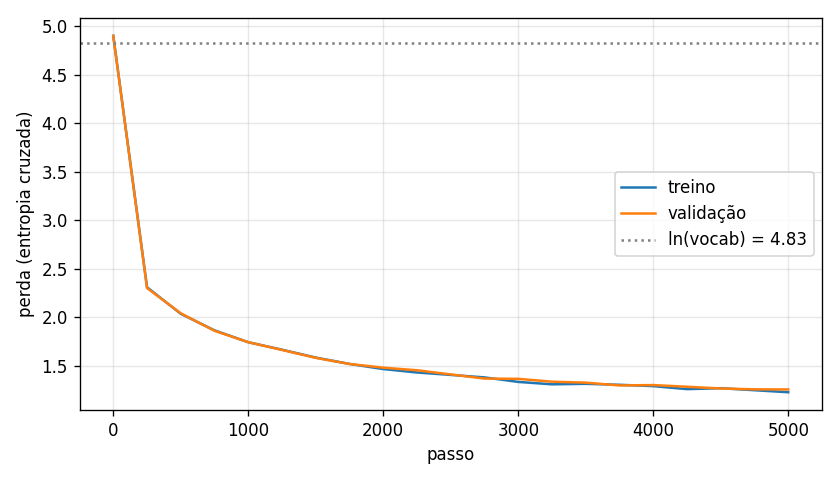
\includegraphics[width=0.8\textwidth]{base/curva_perda.png}
\caption{Curva de perda do modelo base. A linha pontilhada é $\ln 125$.}
\label{fig:curvabase}
\end{figure}

\begin{table}[H]
\centering
\begin{tabular}{@{}rccl@{}}
\toprule
Passo & Treino & Validação & Comparação com os $n$-gramas da Tabela~\ref{tab:ngramas} \\
\midrule
0 & 4,90 & 4,90 & pior que o unigrama (3,24): ainda não sabe nada \\
250 & 2,31 & 2,30 & melhor que o bigrama (2,39) \\
1.000 & 1,74 & 1,74 & entre o trigrama (1,92) e o 4-grama (1,49) \\
2.500 & 1,40 & 1,41 & entre o 4-grama (1,49) e o 5-grama (1,22) \\
5.000 & 1,23 & \textbf{1,25} & perto do 5-grama (1,22); acima do 6-grama (1,14) \\
\bottomrule
\end{tabular}
\caption{Perdas (nats por caractere) ao longo do treino.}
\label{tab:treino}
\end{table}

\paragraph{Leitura dos resultados.}
\begin{enumerate}
\item \textbf{Sem overfitting.} As curvas de treino e validação ficam juntas até o fim; a diferença final é de 0,03. O modelo não está decorando as questões de treino.
\item \textbf{O modelo ainda não convergiu.} A validação ainda caía no passo 5.000. Em 5.000 passos de $32\times 64 = 2.048$ posições, o modelo viu cerca de 10,2 milhões de posições, ou $\approx 2{,}2$ vezes o conjunto de treino (\emph{épocas}). É pouco treino para um conjunto desse tamanho.
\item \textbf{Em bits:} $1{,}25/\ln 2 \approx 1{,}81$ bits por caractere. Para comparar: Shannon \cite{shannon1951} estimou que humanos, prevendo o próximo caractere de textos em inglês, ficam em torno de 1 bit por caractere.
\end{enumerate}

\begin{atencao}[O Transformer ainda perde para o 6-grama]
Pela Tabela~\ref{tab:ngramas}, um 6-grama por contagem chega a 1,14 nats, e o nosso Transformer base a 1,25. Isso não quer dizer que a arquitetura seja pior. O Transformer enxerga 64 caracteres para trás, e o 6-grama só 5, mas precisaria de mais treino ou mais capacidade para tirar proveito disso. O 6-grama, por outro lado, ``decora'' todas as sequências de 6 caracteres do treino de uma vez só, por contagem. Em relatórios, esse tipo de comparação com uma régua simples é essencial: sem ela, 1,25 pareceria um ótimo número. A Seção~\ref{sec:experimentos} testa se um modelo maior supera a régua.
\end{atencao}

\begin{exercicios}
\begin{enumerate}
\item Por que medimos a perda com \texttt{modelo.eval()}? O que aconteceria com a perda de treino medida se o dropout continuasse ligado?
\item Quantas épocas o modelo veria com 15.000 passos e a mesma configuração?
\item Se a perda de validação começasse a subir enquanto a de treino continua caindo, o que isso indicaria? E qual checkpoint o \texttt{train.py} guardaria?
\end{enumerate}
\end{exercicios}

% =====================================================================
\section{Etapa 4: geração e avaliação}
\label{sec:geracao}
% =====================================================================

\subsection{Amostragem auto-regressiva}

O modelo só prevê o próximo caractere. Para escrever um texto, repetimos: passamos o texto até agora (no máximo os últimos 64 caracteres), pegamos os logits da última posição, sorteamos um caractere a partir do softmax, colamos no fim e voltamos ao começo. É a regra da cadeia~\eqref{eq:cadeia} usada ``ao contrário'': em vez de calcular a probabilidade de um texto, sorteamos um texto da distribuição.

\begin{lstlisting}
for _ in range(n_novos):
    contexto = ids[:, -block_size:]           # só os últimos 64 caracteres
    logits, _ = modelo(contexto)
    logits = logits[:, -1, :] / temperatura    # só a última posição interessa
    if top_k is not None:                      # corta a cauda improvável
        limite = torch.topk(logits, top_k).values[:, [-1]]
        logits = logits.masked_fill(logits < limite, float("-inf"))
    proximo = torch.multinomial(F.softmax(logits, dim=-1), num_samples=1)
    ids = torch.cat([ids, proximo], dim=1)
\end{lstlisting}

\subsection{Temperatura e top-$k$}

\paragraph{Temperatura.} Dividimos os logits por $\tau > 0$ antes do softmax:
\begin{equation}
p_i(\tau) = \frac{e^{z_i/\tau}}{\sum_j e^{z_j/\tau}}.
\end{equation}
Com $\tau=1$, é a distribuição que o modelo aprendeu. Quando $\tau \to 0$, a probabilidade se concentra no maior logit, e o sorteio vira escolha gulosa (sempre o mais provável). Quando $\tau \to \infty$, a distribuição tende à uniforme. Temperatura baixa gera texto seguro e repetitivo; alta gera texto variado e com mais erros.

\paragraph{Top-$k$.} Antes do sorteio, mantemos só os $k$ caracteres mais prováveis e zeramos a probabilidade dos demais \cite{fan2018}. Mesmo quando cada caractere improvável tem probabilidade pequena, juntos eles formam uma ``cauda'' que é sorteada de vez em quando, e é daí que vêm os erros mais estranhos. Holtzman et al. \cite{holtzman} estudam esse problema e mostram que a escolha gulosa, por outro lado, leva a repetições.

\subsection{Resultados}

Para avaliar o texto gerado, medimos a fração das palavras geradas (com 3 letras ou mais) que existem no corpus. Cada valor é a média de 5 amostras de 400 caracteres, a partir de \texttt{\#\#\# Revalida}, com a mesma semente para todas as temperaturas:

\begin{table}[H]
\centering
\begin{tabular}{@{}ccc@{}}
\toprule
Temperatura & Palavras reais & Palavras reais com top-$k=10$ \\
\midrule
0,5 & 89\% & 90\% \\
0,8 & 80\% & 83\% \\
1,0 & 71\% & 72\% \\
1,2 & 57\% & 62\% \\
\bottomrule
\end{tabular}
\caption{Qualidade das amostras do modelo base, por temperatura.}
\label{tab:temperatura}
\end{table}

Exemplo com temperatura 0,8:
\begin{lstlisting}[language={},basicstyle=\ttfamily\footnotesize]
### Revalida 2024 | Terapia coletiva
O paciente de um episódio de relação peso agudo, nas condutas ou a elesão das
enconhecidas. Ao exame físico, mostra-se de albumina tipaneopatose e os pesos em
insuficiências no trace de respectivamente sintomal de diarreia e a fase [...]
(C) resposta utilizada como para episódios dias.
(B) Assinale a apresentar o diagnóstico de processo do venos único o
\end{lstlisting}

\paragraph{O que as amostras mostram.}
\begin{itemize}
\item \textbf{O formato foi aprendido}: cabeçalho com prova, ano e área; enunciado que começa como caso clínico; alternativas; gabarito.
\item \textbf{O conteúdo não faz sentido.} As palavras existem, mas as frases não têm significado médico. Com 64 caracteres de contexto (cerca de 10 palavras) e 833 mil parâmetros, o modelo capta ortografia e sintaxe local, não conhecimento.
\item \textbf{Temperatura baixa repete} expressões (``de saúde de \dots de saúde''), como previsto por \cite{holtzman}.
\item \textbf{O top-$k$ ajuda mais nas temperaturas altas}, em que a cauda da distribuição pesa mais.
\end{itemize}

\begin{atencao}[Limites da métrica e da semente]
A métrica de palavras reais aceita frases sem sentido formadas por palavras reais; ela mede ortografia, não significado. Além disso, com uma amostra só por temperatura, os números oscilavam demais: a temperatura 0,5 chegou a dar \emph{menos} palavras reais que a 0,8. Tirar a média de 5 amostras resolveu. A perplexidade de validação continua sendo a métrica principal, porque é calculada sobre meio milhão de caracteres.
\end{atencao}

\begin{exercicios}
\begin{enumerate}
\item Mostre que, com $\tau \to 0$, $p_i(\tau)$ tende a 1 para o maior logit e a 0 para os demais (suponha um único máximo).
\item Qual é a diferença entre top-$k$ com $k=1$ e temperatura muito baixa?
\item Por que o \texttt{generate.py} corta o contexto em \texttt{ids[:, -block\_size:]}? O que aconteceria sem o corte?
\end{enumerate}
\end{exercicios}

% =====================================================================
\section{Etapa 5: experimento com um modelo maior}
\label{sec:experimentos}
% =====================================================================

Esta etapa tem dois experimentos. O primeiro aumenta o \emph{tamanho} do modelo; o segundo, o \emph{contexto} que ele enxerga. Em cada um, mudamos uma coisa só e mantemos todo o resto igual, para saber a que atribuir a diferença.

\subsection{Experimento 1: um modelo maior}

\paragraph{Pergunta e hipótese.}

O modelo base não teve overfitting e ainda perdia para o 6-grama. Quando treino e validação andam juntos, o modelo provavelmente tem \emph{pouca capacidade} para os dados: ele não consegue nem decorar o treino. A hipótese é que um modelo maior chegue a uma perda menor. Kaplan et al. \cite{kaplan} mediram que, em modelos de linguagem, a perda cai de forma previsível (uma lei de potência) conforme crescem o número de parâmetros, a quantidade de dados e o cálculo gasto no treino.

\paragraph{Montagem do experimento.}

Para a comparação ser justa, mudamos \textbf{só o tamanho} do modelo. Passos, lote, contexto, taxa de aprendizado, dropout e semente ficaram iguais aos da base (\texttt{configs/grande.json}):

\begin{table}[H]
\centering
\begin{tabular}{@{}lcc@{}}
\toprule
 & Base & Grande \\
\midrule
\texttt{n\_embd} ($C$) & 128 & 256 \\
\texttt{n\_head} (dimensão por cabeça) & 4 (32) & 8 (32) \\
\texttt{n\_layer} & 4 & 6 \\
Parâmetros & 833.661 & 4.819.581 (5,8$\times$) \\
Tempo por passo na CPU & $\approx 0{,}15$ s & $\approx 0{,}44$ s \\
Tempo total (5.000 passos) & 12,7 min & 47,6 min \\
\bottomrule
\end{tabular}
\caption{Configurações comparadas. O restante é igual: contexto 64, lote 32, $\eta = 10^{-3}$, dropout 0,1.}
\end{table}

Pela Tabela~\ref{tab:parametros}, cada bloco tem $\approx 12C^2$ parâmetros. Dobrar $C$ multiplica cada bloco por 4, e passar de 4 para 6 blocos multiplica por mais 1,5: daí o fator $\approx 6$.

\paragraph{Resultados.}

Além da estimativa com 100 lotes feita durante o treino, medimos os dois modelos finais no conjunto de validação \emph{inteiro} (508.160 posições), para a comparação com os $n$-gramas ser feita nos mesmos dados:

\begin{table}[H]
\centering
\small
\begin{tabular}{@{}lccccc@{}}
\toprule
Modelo & Perda val. & Bits/caractere & Perplexidade & Treino $-$ val. & Palavras reais \\
\midrule
Unigrama & 3,235 & 4,67 & 25,4 & -- & -- \\
5-grama & 1,223 & 1,76 & 3,40 & -- & -- \\
6-grama & 1,142 & 1,65 & 3,13 & -- & -- \\
Transformer base & 1,249 & 1,80 & 3,49 & $-0{,}029$ & 80\% \\
\textbf{Transformer grande} & \textbf{1,124} & \textbf{1,62} & \textbf{3,08} & $-0{,}036$ & \textbf{87\%} \\
\bottomrule
\end{tabular}
\caption{Validação inteira. ``Treino $-$ val.'' é a diferença no último passo (negativa: o treino vai melhor). Palavras reais: média de 5 amostras a $\tau=0{,}8$, com a mesma semente para os dois modelos (\texttt{compare.py}).}
\label{tab:experimento}
\end{table}

\begin{figure}[H]
\centering
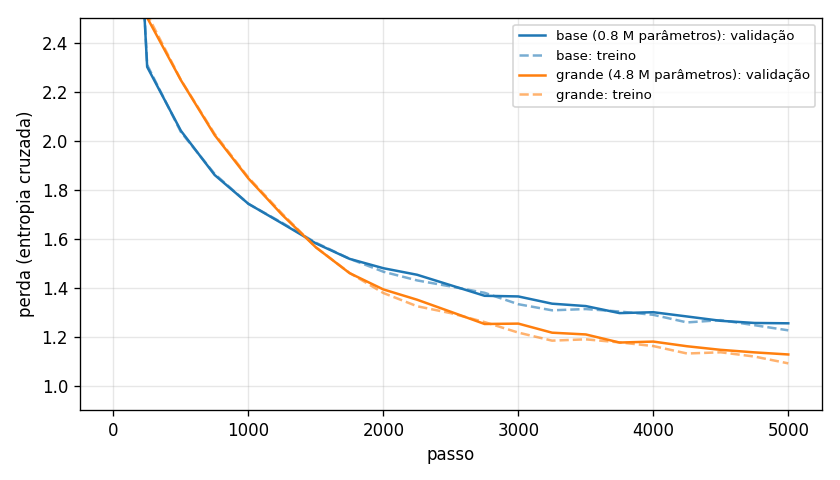
\includegraphics[width=0.8\textwidth]{comparacao.png}
\caption{Curvas de perda dos dois modelos. Linha cheia: validação; tracejada: treino. O eixo vertical foi cortado em 2,5 para mostrar a parte final.}
\label{fig:comparacao}
\end{figure}

\paragraph{Leitura dos resultados.}
\begin{enumerate}
\item \textbf{A hipótese se confirmou.} O modelo grande terminou com perda 0,125 nats menor (1,124 contra 1,249). Em probabilidade média no caractere certo: $e^{-1{,}124} \approx 32{,}5\%$ contra $e^{-1{,}249} \approx 28{,}7\%$.
\item \textbf{O Transformer passou do 6-grama, mas por pouco}: 1,124 contra 1,142. Dois detalhes deixam a comparação ainda mais apertada. A suavização do 6-grama foi escolhida olhando a validação, o que o favorece. Por outro lado, na medição do Transformer, as posições do começo de cada janela de 64 caracteres têm pouco contexto, o que o desfavorece.
\item \textbf{O modelo grande começa mais devagar.} Até o passo $\approx 1.500$, ele fica \emph{acima} da base (Figura~\ref{fig:comparacao}). Com a mesma taxa de aprendizado, um modelo com mais parâmetros precisa de mais passos até organizar suas representações. Depois disso, ele passa a base e a distância só aumenta.
\item \textbf{Com o mesmo tempo de CPU, a base ganha.} Aos 13 minutos, quando a base já tinha terminado com 1,25, o grande estava por volta do passo 1.300, com perda $\approx 1{,}65$. ``Qual modelo é melhor'' depende da pergunta: com o mesmo número de passos, o grande; com o mesmo orçamento de cálculo curto, o pequeno. Hoffmann et al. \cite{hoffmann} estudam exatamente como dividir um orçamento de cálculo entre tamanho do modelo e quantidade de dados.
\item \textbf{O começo de uma separação entre treino e validação.} A diferença final passou de $-0{,}029$ para $-0{,}036$, e no passo 5.000 o treino (1,09) está visivelmente abaixo da validação (1,13). Ainda é pequena, mas é o primeiro sinal de que o modelo maior tem capacidade para começar a decorar. Com mais passos, o dropout e o conjunto de validação passam a ser essenciais.
\item \textbf{Amostras um pouco melhores.} A taxa de palavras reais subiu de 80\% para 87\%. O conteúdo continua sem sentido médico:
\end{enumerate}

\begin{lstlisting}[language={},basicstyle=\ttfamily\footnotesize]
### Revalida 2014
Uma mulher com 44 anos de idade, sem prevenção de mecânio anti-hipertenso. Em
sinais de esclerose impulsiva em espectronente quadro de possa albumina tipa e
pancreática pelo membro inferior de nefrologia à segmentação;
(E) onda endoscopia hormonal do manijor de atenção acessociada a que, está visar
\end{lstlisting}

\begin{atencao}[O que este experimento não mostra]
Fizemos \textbf{um} treino de cada modelo, com \textbf{uma} semente. Parte da diferença pode vir da sorte na inicialização e na ordem dos lotes. Para afirmar com segurança que o grande é melhor, o ideal seria repetir cada treino com 3 sementes e comparar médias e desvios. Aqui, a diferença (0,125 nats) é bem maior que as oscilações entre avaliações vizinhas da mesma curva (cerca de 0,01 a 0,03), o que torna o resultado plausível, mas não o prova.
\end{atencao}

\subsection{Uma correção na forma de medir}

Até aqui, a perda na validação inteira foi medida com janelas de 64 caracteres \emph{lado a lado}. Nelas, o primeiro caractere de cada janela é previsto sem contexto nenhum, o segundo com 1 caractere, e assim por diante: em média, cada previsão usa só 32 caracteres de contexto. Isso subestima o modelo e, pior, torna injusta a comparação entre modelos com contextos diferentes.

A medida correta usa uma \textbf{janela deslizante}: as janelas andam meio contexto por vez e só a segunda metade de cada uma entra na conta. Assim, todo caractere é previsto com pelo menos metade do contexto do modelo. Esse é o método do \texttt{compare.py} a partir daqui. O 6-grama não muda, porque sempre usa os 5 caracteres anteriores.

\begin{table}[H]
\centering
\begin{tabular}{@{}lcc@{}}
\toprule
Modelo & Janelas lado a lado & Janela deslizante \\
\midrule
Transformer base & 1,249 & 1,193 \\
Transformer grande & 1,124 & 1,055 \\
6-grama (referência) & \multicolumn{2}{c}{1,142} \\
\bottomrule
\end{tabular}
\caption{A mesma validação, medida das duas formas. Com a medida correta, o modelo grande passa o 6-grama com folga (1,055 contra 1,142), e não ``por pouco''.}
\end{table}

\subsection{Experimento 2: mais contexto}

\paragraph{Pergunta e hipótese.} As amostras do modelo grande pareciam ``pedaços colados'': cada trecho fazia sentido com a linha anterior, mas o texto perdia o fio. Em 5 amostras de 600 caracteres do modelo grande, medimos que 18\% a 46\% do texto gerado são trechos de 20 ou mais caracteres idênticos ao corpus, mas nenhum passa de 42 caracteres: são as fórmulas das provas (``Assinale a opção que indica''), não questões copiadas. A explicação provável é o contexto de 64 caracteres, cerca de uma linha. A hipótese: com 128 caracteres, o modelo mantém melhor a estrutura da questão.

\paragraph{Montagem.} Igual ao modelo grande, mudando só \texttt{block\_size} de 64 para 128 (\texttt{configs/contexto.json}). A embedding de posição cresce de 64 para 128 linhas, e o modelo passa a ter 4.835.965 parâmetros. Cada passo processa o dobro de caracteres, e o custo da atenção cresce com o quadrado do contexto. O treino levou \textbf{120 minutos} na CPU, contra 48 do grande.

\paragraph{Uma medida de coerência.} Para testar diretamente se o modelo ``lembra'' o que escreveu, contamos, dentro de cada questão gerada, os pares de alternativas seguidas e quantos estão em ordem: \texttt{(A)} depois \texttt{(B)}, \texttt{(B)} depois \texttt{(C)}. Para acertar, o modelo precisa lembrar a letra da alternativa anterior, que muitas vezes está a mais de 64 caracteres de distância. Geramos 90 textos de 1.000 caracteres por modelo, a partir de \texttt{\#\#\# Revalida}, com temperatura 0,8.

\paragraph{Resultados.}

\begin{table}[H]
\centering
\small
\begin{tabular}{@{}lccccc@{}}
\toprule
Modelo & Contexto & Perda (deslizante) & Perplexidade & Alternativas em ordem & Tempo \\
\midrule
6-grama & 5 & 1,142 & 3,13 & -- & -- \\
Base & 64 & 1,193 & 3,30 & -- & 13 min \\
Grande & 64 & 1,055 & 2,87 & 42,7\% (76/178) & 48 min \\
\textbf{Contexto} & \textbf{128} & \textbf{1,015} & \textbf{2,76} & \textbf{74,6\% (94/126)} & 120 min \\
\bottomrule
\end{tabular}
\caption{Os dois experimentos, com a medida correta de perda.}
\label{tab:contexto}
\end{table}

\begin{enumerate}
\item \textbf{A perda caiu de 1,055 para 1,015.} É uma melhora menor que a do Experimento 1, mas vem só do contexto: o número de parâmetros é praticamente o mesmo.
\item \textbf{A coerência melhorou muito}: de 42,7\% para 74,6\% das alternativas em ordem. Um teste de diferença entre duas proporções dá $z \approx 5{,}5$; uma diferença desse tamanho por acaso é praticamente impossível. Esse é o efeito que a perda média esconde: a maioria dos caracteres depende só das letras vizinhas, e o contexto longo importa em poucos pontos, justamente os que dão estrutura ao texto.
\item \textbf{O modelo com mais contexto começa muito mais devagar.} Até o passo $\approx 1.000$, a perda dele fica quase parada entre 2,5 e 2,3, acima dos outros dois. Depois ela cai rápido e passa a do grande por volta do passo 2.750.
\item \textbf{O custo é alto}: 2,5 vezes o tempo do grande, para 0,04 nats a menos. Para um orçamento fixo de tempo, pode valer mais treinar o grande por mais passos.
\end{enumerate}

\subsection{Próximos experimentos sugeridos}

\begin{itemize}
\item \textbf{Treinar o modelo de contexto 128 por mais passos} (10.000 a 15.000), com taxa de aprendizado decrescente, acompanhando a separação entre treino e validação.
\item \textbf{Contexto 256}, idealmente na GPU, já que o custo da atenção cresce com o quadrado do contexto.
\item \textbf{Repetir com sementes diferentes}, para medir a variação entre treinos.
\item \textbf{Treinar na GPU do Kaggle}, que deve ser dezenas de vezes mais rápida que a CPU para esse tamanho de modelo.
\end{itemize}

\begin{exercicios}
\begin{enumerate}
\item Usando $\approx 12C^2$ por bloco, estime os parâmetros de um modelo com $C=384$ e 6 blocos. Quanto tempo por passo você espera na CPU, supondo que o tempo cresce na mesma proporção que os parâmetros?
\item Por que medir no conjunto de validação inteiro é mais confiável que a média de 100 lotes sorteados? Quantas posições cada uma das duas medições usa?
\item Se o treino do modelo grande continuasse até a validação parar de cair, qual checkpoint o \texttt{train.py} guardaria? Por que isso protege contra o overfitting?
\end{enumerate}
\end{exercicios}


% =====================================================================
\section{Resumo e próximos passos}
% =====================================================================

\begin{enumerate}
\item \textbf{Dados.} Limpar o texto (NFC, homóglifos, símbolos equivalentes e raros) reduziu o vocabulário de 144 para 125 caracteres sem mudar o sentido. A separação por questão evita vazamento entre treino e validação.
\item \textbf{Arquitetura.} Um Transformer só com decoder: embeddings de token e posição, blocos com atenção causal e MLP, conexões residuais e LayerNorm pre-norm. A perda inicial de 4,90, perto de $\ln 125 = 4{,}83$, e os testes de causalidade e de ``decorar um lote'' confirmam a implementação.
\item \textbf{Treino.} AdamW com dropout, avaliação periódica e checkpoint do melhor modelo. O modelo base chega a 1,25 nats por caractere, sem overfitting e ainda sem ter convergido.
\item \textbf{Geração.} O modelo aprende o \emph{formato} das questões, mas não o \emph{conteúdo}. A temperatura controla a troca entre acerto e variedade.
\item \textbf{Régua.} Um 6-grama por contagem (1,14) supera o modelo base. Comparar com uma régua simples é o que dá sentido aos números.
\item \textbf{Escala.} Com 5,8 vezes mais parâmetros e os mesmos 5.000 passos, a perda caiu para 1,12, passando o 6-grama por pouco. O modelo maior começa mais devagar, custa 3,7 vezes mais tempo e mostra o primeiro sinal de separação entre treino e validação.
\end{enumerate}

Ideias para continuar: treinar por mais passos, com uma taxa de aprendizado que decai ao longo do treino (\emph{cosine schedule}); aumentar o contexto (\texttt{block\_size} 128 ou 256); repetir os treinos com outras sementes; trocar a tokenização por BPE \cite{sennrich}; treinar na GPU do Kaggle.

\begin{thebibliography}{99}
\bibitem{goodfellow} I.~Goodfellow, Y.~Bengio e A.~Courville. \emph{Deep Learning}. MIT Press, 2016. Disponível em \url{https://www.deeplearningbook.org}.
\bibitem{jurafsky} D.~Jurafsky e J.~H.~Martin. \emph{Speech and Language Processing}, 3.ª ed. (rascunho). Disponível em \url{https://web.stanford.edu/~jurafsky/slp3/}.
\bibitem{cover} T.~M.~Cover e J.~A.~Thomas. \emph{Elements of Information Theory}, 2.ª ed. Wiley, 2006.
\bibitem{bishop} C.~M.~Bishop e H.~Bishop. \emph{Deep Learning: Foundations and Concepts}. Springer, 2024.
\bibitem{vaswani} A.~Vaswani et al. Attention Is All You Need. \emph{NeurIPS}, 2017.
\bibitem{radford2019} A.~Radford et al. Language Models are Unsupervised Multitask Learners (GPT-2). OpenAI, 2019.
\bibitem{karpathy} A.~Karpathy. \emph{Let's build GPT: from scratch, in code, spelled out} (vídeo) e repositório nanoGPT. 2023. \url{https://github.com/karpathy/nanoGPT}.
\bibitem{bengio2003} Y.~Bengio, R.~Ducharme, P.~Vincent e C.~Jauvin. A Neural Probabilistic Language Model. \emph{JMLR}, 3:1137--1155, 2003.
\bibitem{shannon1951} C.~E.~Shannon. Prediction and Entropy of Printed English. \emph{Bell System Technical Journal}, 30(1):50--64, 1951.
\bibitem{sennrich} R.~Sennrich, B.~Haddow e A.~Birch. Neural Machine Translation of Rare Words with Subword Units. \emph{ACL}, 2016.
\bibitem{he2016} K.~He, X.~Zhang, S.~Ren e J.~Sun. Deep Residual Learning for Image Recognition. \emph{CVPR}, 2016.
\bibitem{layernorm} J.~L.~Ba, J.~R.~Kiros e G.~E.~Hinton. Layer Normalization. arXiv:1607.06450, 2016.
\bibitem{gelu} D.~Hendrycks e K.~Gimpel. Gaussian Error Linear Units (GELUs). arXiv:1606.08415, 2016.
\bibitem{dropout} N.~Srivastava et al. Dropout: A Simple Way to Prevent Neural Networks from Overfitting. \emph{JMLR}, 15:1929--1958, 2014.
\bibitem{adam} D.~P.~Kingma e J.~Ba. Adam: A Method for Stochastic Optimization. \emph{ICLR}, 2015.
\bibitem{adamw} I.~Loshchilov e F.~Hutter. Decoupled Weight Decay Regularization. \emph{ICLR}, 2019.
\bibitem{fan2018} A.~Fan, M.~Lewis e Y.~Dauphin. Hierarchical Neural Story Generation. \emph{ACL}, 2018.
\bibitem{holtzman} A.~Holtzman et al. The Curious Case of Neural Text Degeneration. \emph{ICLR}, 2020.
\bibitem{kaplan} J.~Kaplan et al. Scaling Laws for Neural Language Models. arXiv:2001.08361, 2020.
\bibitem{hoffmann} J.~Hoffmann et al. Training Compute-Optimal Large Language Models. \emph{NeurIPS}, 2022.
\bibitem{healthqa} HealthQA-BR. Conjunto de dados no Hugging Face: \url{https://huggingface.co/datasets/Larxel/healthqa-br}. Licença CC-BY 4.0.
\end{thebibliography}

\end{document}
